\chapter{Автоматическое дифференцирование}
\label{chap:automatic_differentiation}

\begin{supportbox}{Об этой главе}
Предыдущая глава подчеркнула необходимость эффективной, автоматической процедуры для вычисления градиентов любой возможной последовательности операций. В этой главе мы описываем такой метод, называемый \textbf{обратным распространением ошибки} в литературе по нейронным сетям или \textbf{автоматическим дифференцированием в обратном режиме} в компьютерных науках. Его анализ дает несколько идей, от выбора модели до требований к памяти для ее оптимизации.
\end{supportbox}

\section{Постановка задачи}

Мы рассматриваем задачу эффективного вычисления градиентов общих \textit{вычислительных графов}, таких как те, что возникают при оптимизации скалярной функции потерь на полносвязной модели, задача, называемая \textbf{автоматическим дифференцированием} (АД) \cite{baydin2018automatic}. Вы можете думать о вычислительном графе как о наборе атомарных операций (которые мы называем \textbf{примитивами}), полученных при выполнении самой программы. Для краткости мы будем рассматривать последовательные графы, но все можно легко расширить на ациклические и даже более общие вычислительные графы \cite{griewank2008evaluating,blondel2024elements} .

Задача может показаться тривиальной, поскольку цепное правило Якобианов (Раздел \ref{sec:gradients_and_jacobians}, \eqref{eq:jacobian_chain_rule}) говорит нам, что градиент композиции функций — это просто произведение матриц соответствующих Якобианов. Однако эффективная реализация этого является ключевой задачей, и результирующий алгоритм (\textbf{АД в обратном режиме} или \textbf{обратное распространение ошибки}) является краеугольным камнем нейронных сетей и дифференцируемого программирования в целом \cite{griewank2008evaluating,blondel2024elements}. Понимание его также является ключом к пониманию дизайна (и различий) большинства фреймворков для реализации и обучения таких программ (таких как TensorFlow, PyTorch или JAX). Краткую историю алгоритма можно найти в \cite{griewank2012invented}.

Для постановки задачи мы предполагаем, что в нашем распоряжении есть набор \textbf{примитивов}:
%
$$\mathbf{y} =f_i(\mathbf{x}, \mathbf{w}_i)$$
%
Каждый примитив представляет собой операцию над входным вектором $\mathbf{x} \sim ({c_i})$, параметризованную вектором $\mathbf{w}_i \sim (p_i)$ (например, весами линейной проекции), и дающую на выходе другой вектор $\mathbf{y} \sim (c^\prime_i)$.

В нашем определении примитивов есть большая гибкость, они могут представлять базовые операции линейной алгебры (например, умножение матриц), слои в смысле Главы \ref{chap:fully_connected_models} (например, полносвязный слой с функцией активации) или даже более крупные блоки или модели. Эта рекурсивная композиционность является ключевым свойством программирования и распространяется на наш случай.

Мы предполагаем только, что для каждого примитива мы знаем, как вычислить частные производные по двум входным аргументам, которые мы называем \textbf{входным Якобианом} и \textbf{весовым Якобианом} операции:
%
\begin{eqnarray*}
\textbf{Входной Якобиан: } & \partial_{\mathbf{x}}\left[f(\mathbf{x},\mathbf{w})\right] \sim (c^\prime,c) \\
\textbf{Весовой Якобиан: } & \partial_{\mathbf{w}}\left[f(\mathbf{x},\mathbf{w})\right] \sim (c^\prime,p) 
\end{eqnarray*}

Это разумные предположения, поскольку мы ограничиваем наш анализ дифференцируемыми моделями. Непрерывные примитивы с одной или несколькими точками недифференцируемости, такие как ReLU, могут быть вписаны в эту структуру с использованием \textbf{субградиентов} (Раздел \ref{subsec:subdifferentiability}). Недифференцируемые операции, такие как выборка или пороговое значение, также могут быть включены путем нахождения релаксации их градиента или эквивалентного оценщика \cite{niculae2023discrete}. Последний случай мы рассмотрим в следующем томе.
%
\subsection*{О нашей нотации и Якобианах высшего порядка}

\addteacup Для удобочитаемости мы рассматриваем только векторнозначные величины, поскольку все результирующие градиенты являются матрицами. На практике существующие примитивы могут иметь входы, веса или выходы более высокого ранга. Например, рассмотрим базовый полносвязный слой на входе с мини-пакетом:
%
$$
f(\mathbf{X},\mathbf{W})=\mathbf{X}\mathbf{W}+\mathbf{b}
$$
%
В этом случае вход $\mathbf{X}$ имеет форму $(n,c)$, веса имеют форму $(c,c’)$ и $(c^\prime)$ (где $c^\prime$ — гиперпараметр), а выход имеет форму $(n, c^\prime)$. Следовательно, входной Якобиан имеет форму $(n,c^\prime, n, c)$, а весовой Якобиан имеет форму $(n,c^\prime, c, c^\prime)$, оба имеют ранг $4$. 

В нашей нотации мы можем рассмотреть эквивалентные уплощенные векторы $\mathbf{x} = \text{vect}(\mathbf{X})$ и $\mathbf{w} = \left[\text{vect}(\mathbf{W}); \mathbf{b}\right]$, и наши результирующие «уплощенные» Якобианы имеют форму $(nc^\prime, nc)$ и $(nc^\prime, cc^\prime)$ соответственно. Это крайне важно в дальнейшем, поскольку каждый раз, когда мы ссылаемся на «\textit{размер входа $c$}» мы имеем в виду «\textit{произведение всех форм входа}», включая возможные размеры мини-пакетов. Это также показывает, что, хотя мы можем знать, как вычислять Якобианы, мы можем не захотеть полностью \textit{материализовать} их в памяти из-за их большой размерности.

В качестве заключительного замечания, наша нотация согласуется с тем, как эти примитивы реализованы в функциональной библиотеке, такой как JAX. В объектно-ориентированном фреймворке (например, TensorFlow, PyTorch) мы видели,
что слои реализованы как объекты (см. Листинг \ref{code:fully_connected_layer} в предыдущей главе), где параметры являются свойством объекта, а вызов функции заменяется методом объекта. Этот стиль упрощает определенные практики, такие как отложенная инициализация всех параметров до тех пор, пока не станут известны формы входа (\textbf{ленивая инициализация}), но он добавляет небольшой слой абстракции, который необходимо учитывать для перевода нашей нотации в рабочий код. Как мы увидим, эти различия, в свою очередь, отражаются в том, как АД реализовано в двух фреймворках.

\subsection{Автоматическое дифференцирование: постановка задачи}

Со всеми этими деталями мы готовы сформулировать задачу АД. Рассмотрим последовательность из $l$ вызовов примитивов, за которой следует итоговое суммирование:
%
\begin{eqnarray*}
\mathbf{h}_1 & = & f_1(\mathbf{x}, \mathbf{w}_1) \\
\mathbf{h}_2 & = & f_2(\mathbf{h}_1, \mathbf{w}_2) \\
& \vdots &  \\
\mathbf{h}_{l} & = & f_{l}(\mathbf{h}_{l-1}, \mathbf{w}_{l}) \\
y & = & \sum \mathbf{h}_{l} 
\end{eqnarray*}
%
Это называется \textbf{трассой вычислений} программы. Грубо говоря, первые $l-1$ операций могут представлять несколько слоев дифференцируемой модели, операция $l$ может быть потерей для каждого входа (например, кросс-энтропия), а последняя операция суммирует потери мини-пакета. Следовательно, выход нашей программы всегда является скаляром, поскольку это требуется для численной оптимизации. Мы сокращаем предыдущую программу как $F(\mathbf{x})$. 

\begin{definition}[Автоматическое дифференцирование] \addbottle
%
Для программы $F(\mathbf{x})$, состоящей из последовательности дифференцируемых примитивов, \textbf{автоматическое дифференцирование} (АД) относится к задаче \textit{одновременного} и \textit{эффективного} вычисления всех весовых Якобианов программы при знании вычислительного графа и всех индивидуальных входных и весовых Якобианов:
%
$$\text{AD}(F(\mathbf{x}))=\left\{\partial_{\mathbf{w}_i} y\right\}_{i=1}^{l}$$
\end{definition}
%
Как мы увидим, существует два основных класса алгоритмов АД, называемых \textbf{прямым режимом} и \textbf{обратным режимом}, соответствующих разному порядку композиции отдельных операций. Мы также увидим, что обратный режим (называемый \textbf{обратным распространением ошибки} в литературе по нейронным сетям) значительно более эффективен в нашем контексте. Хотя мы сосредоточимся на упрощенном сценарии, относительно легко расширить наш вывод на ациклические графы примитивов (как уже упоминалось), а также на ситуации, когда параметры разделяются между слоями (\textbf{разделение весов}). Мы увидим пример разделения весов в Главе \ref{chap:rnns}.

\subsection{Численное и символьное дифференцирование}

\addteacup Прежде чем перейти к АД в прямом режиме, мы прокомментируем разницу между АД и другими классами алгоритмов для дифференцирования функций. Во-первых, мы могли бы напрямую применить определение градиентов (Раздел \ref{sec:gradients_and_jacobians}), чтобы получить подходящее численное приближение градиента. Этот процесс называется \textbf{численным дифференцированием}. Однако каждое скалярное значение, которое нужно дифференцировать, требует 2 вызовов функции в наивной реализации, что делает этот подход невозможным, за исключением численных проверок реализации.

Во-вторых, рассмотрим эту простую функцию:
%
$$
f(x)=a\sin(x)+bx\sin(x)
$$
%
Мы можем попросить символьный движок предварительно вычислить полное, символьное уравнение производной. Это называется \textbf{символьным дифференцированием} и показано на Python в Листинге \ref{code:symbolic_differentiation}.

В реалистичной реализации промежуточное значение $h=\sin(x)$ будет вычислено только один раз и сохранено в промежуточной переменной, которая также может быть повторно использована для соответствующего вычисления в трассе градиента (и аналогичное рассуждение относится к члену $\cos(x)$ в производной). Это менее тривиально, чем кажется: нахождение оптимальной реализации для Якобиана, которая избегает любых ненужных вычислений, является NP-полной задачей (\textbf{оптимальное накопление Якобиана}). Однако мы увидим, что можем использовать структуру нашей программы для разработки достаточно эффективной реализации АД, которая значительно лучше, чем символьный подход, подобный приведенному выше (и на самом деле эквивалентна символьному подходу, допускающему наличие подпоследовательностей \cite{laue2019equivalence}).

\begin{mypy}{Символьное дифференцирование на Python с использованием SymPy.}{code:symbolic_differentiation}
import sympy as sp
x, a, b = sp.symbols('x a b')
y = a*sp.sin(x) + b*x*sp.sin(x)
sp.diff(y, x) # [Out]: acos(x)+bxcos(x)+bsin(x)
\end{mypy}

\section{Автоматическое дифференцирование в прямом режиме}

Начнем с напоминания о цепном правиле Якобианов. Рассмотрим комбинацию двух примитивных функций:
%
$$\mathbf{h}=f_1(\mathbf{x)} \;,\; \mathbf{y}=f_2(\mathbf{h})$$
%
В терминах их градиентов мы имеем:
%
$$\partial_{\mathbf{x}}\,\mathbf{y} = {\color{drawgreen}\partial_{\mathbf{h}} \,\mathbf{y}} \,\cdot\,\!{\color{drawred}\partial_{\mathbf{x}}\,\mathbf{h}}$$
%
Если $\mathbf{x}$, $\mathbf{h}$ и $\mathbf{y}$ имеют размерности $a$, $b$ и $c$ соответственно, предыдущий Якобиан требует умножения матрицы $c \times b$ (зеленым) на матрицу $b \times a$ (красным). Мы можем интерпретировать это правило следующим образом: если мы уже вычислили $f_1$ и ее Якобиан (красный член), как только мы применим $f_2$, мы можем «обновить» градиент, умножив на соответствующий Якобиан (зеленый член).

Мы можем немедленно применить это понимание для получения работающего алгоритма, называемого \textbf{автоматическим дифференцированием в прямом режиме} (F-AD). Идея заключается в том, что каждый раз, когда мы применяем примитивную функцию, мы инициализируем ее соответствующий весовой Якобиан (называемый \textbf{касательной} в этом контексте), одновременно обновляя все предыдущие касательные матрицы. Давайте рассмотрим простой проработанный пример, чтобы проиллюстрировать основной алгоритм.

Рассмотрим первую инструкцию, $\mathbf{h}_1 = f_1(\mathbf{x}, \mathbf{w}_1)$, в нашей программе. Поскольку до сих пор ничего не было сохранено, мы инициализируем касательную матрицу для $\mathbf{w}_1$ как ее весовой Якобиан:

$$\widehat{\mathbf{W}}_1 = \partial_{\mathbf{w}_1} \, \mathbf{h}_1$$

Мы теперь переходим ко второй инструкции, $\mathbf{h}_2 = f_2(\mathbf{h}_1, \mathbf{w}_2)$. Мы обновляем предыдущую касательную матрицу, одновременно инициализируя вторую:

\begin{gather*}
\eqnmarkbox[drawgreen]{node2}{\widehat{\mathbf{W}}_1} \leftarrow \eqnmarkbox[drawred]{node}{\left[\partial_{\mathbf{h}_1} \mathbf{h}_2\right]} \widehat{\mathbf{W}}_1 \\
\widehat{\mathbf{W}}_2 = \partial_{\mathbf{w}_2}\,\mathbf{h}_2
\end{gather*}
\annotate[yshift=1em]{above,right}{node}{Входной Якобиан $f_2$}
\annotate[yshift=1em]{above,left}{node2}{Обновленная касательная матрица для $\mathbf{w}_1$}

\vspace{-2em}
Обновление требует входного Якобиана примитива, в то время как второй член требует весового Якобиана примитива. Абстрагируясь, рассмотрим общий $i$-й примитив, заданный как $\mathbf{h}_i = f_i(\mathbf{h}_{i-1}, \mathbf{w}_i)$. Мы инициализируем касательную матрицу для $\mathbf{w}_i$, одновременно обновляя \textit{все} предыдущие матрицы:

\begin{gather*}
\widehat{\mathbf{W}}_j \leftarrow \left[\eqnmarkbox[drawred]{node}{\partial_{\mathbf{h}_{i-1}} \mathbf{h}_i}\right] \widehat{\mathbf{W}}_j \;\; \forall j <i \\
\widehat{\mathbf{W}}_i = \eqnmarkbox[drawgreen]{node2}{\partial_{\mathbf{w}_i}}\,\mathbf{h}_i
\end{gather*}
\annotate[yshift=1em]{above,right}{node}{Входной Якобиан $f_i$}
\annotate[yshift=-1em]{below,right}{node2}{Весовой Якобиан $f_i$}

\vspace{1em}
В первой строке $i-1$ обновлений (по одному для каждой касательной матрицы, которую мы уже сохранили в памяти), причем красный член — входной Якобиан $i$-й операции — является общим для всех предыдущих касательных. Последняя операция в программе — это сумма, и соответствующий градиент дает нам выход алгоритма:\footnote{Чтобы быть полностью последовательными с нотацией, выход \eqref{eq:last_step_fad} — это вектор-строка, в то время как мы определили градиент как вектор-столбец. Мы будем игнорировать этот тонкий момент для простоты, пока не придет время определить векторно-якобианские произведения позже в главе.}

\begin{equation}
\nabla_{\mathbf{w}_i}y=  \mathbf{1}^\top\widehat{\mathbf{W}}_i \;\; \forall i
\label{eq:last_step_fad}
\end{equation}

Готово! Давайте проанализируем алгоритм более подробно. Во-первых, все перечисленные нами операции можно легко \textit{чередовать} с исходной программой, что означает, что пространственная сложность будет примерно пропорциональна пространственной сложности дифференцируемой программы.

С отрицательной стороны, основная операция алгоритма (обновление $\widehat{\mathbf{W}}_i$) требует умножения двух матриц, в общем случае имеющих формы $(c^\prime_i, c_i)$ и $(c_i, p_j)$, где $c_i, c^\prime_i$ — это формы входа/выхода, а $p_j$ — форма $\mathbf{w}_j$. Это чрезвычайно дорогостоящая операция: например, предположим, что входы и выходы имеют форму $(n,d)$, где $n$ — размер мини-пакета, а $d$ — количество признаков. Тогда умножение матриц будет иметь сложность $\mathcal{O}(n^2d^2p_j)$, что является квадратичным как по размеру мини-пакета, так и по размерности признаков. Это может легко стать невозможным, особенно для высокоразмерных входов, таких как изображения.

Мы можем получить лучший компромисс, заметив, что последняя операция алгоритма — это более простое произведение матрицы на вектор, что является следствием наличия скалярного выхода. Это более подробно рассматривается в следующем разделе.

\section{Автоматическое дифференцирование в обратном режиме}
\label{sec:reverse_mode_automatic_differentiation}

\addclock Чтобы продолжить, мы развернем вычисление одного члена градиента, соответствующего $i$-й весовой матрице:
%
\begin{equation}
\nabla_{\mathbf{w}_i}\,y = \mathbf{1}^\top {\color{drawred}\left[ \partial_{\mathbf{h}_{l-1}}\,\mathbf{h}_{l}\right] \cdots \left[ \partial_{\mathbf{h}_{i}}\,\mathbf{h}_{i+1}\right]} {\color{drawgreen}\left[ \partial_{\mathbf{w}_{i}}\,\mathbf{h}_{i}\right]}
\label{eq:backward_pass}
\end{equation}
%
Помните, что, не считая нотации, \eqref{eq:backward_pass} — это просто потенциально длинная серия умножений матриц, включающая постоянный член (вектор $\mathbf{1}$ из единиц), серию входных Якобианов (красный член) и весовой Якобиан соответствующей весовой матрицы (зеленый член). Давайте определим сокращение для красного члена:
%
\begin{equation}
    \widetilde{\mathbf{h}}_i = \mathbf{1}^\top \prod_{j=i+1}^{l} \partial_{\mathbf{h}_{j-1}}\,\mathbf{h}_{j}
    \label{eq:recursive_h}
\end{equation}
%
Поскольку умножение матриц ассоциативно, мы можем выполнять вычисления в \eqref{eq:backward_pass} в любом порядке. В F-AD мы двигались справа налево, поскольку это соответствует порядку, в котором выполнялись примитивные функции. Однако мы можем сделать лучше, заметив два интересных аспекта:

\begin{enumerate}
\item Крайний левый член в \eqref{eq:backward_pass} — это произведение вектора на матрицу (что является следствием наличия скалярного члена на выходе), что вычислительно лучше, чем произведение двух матриц. Его выход также является другим вектором.
\item Член в \eqref{eq:recursive_h} (произведение всех входных Якобианов от слоя $i$ до слоя $l$) можно вычислить рекурсивно, начиная с \textit{последнего} члена и итеративно умножая на входные Якобианы в обратном порядке.
\end{enumerate}

Мы можем объединить эти наблюдения для разработки второго подхода к автоматическому дифференцированию, который мы назовем \textbf{автоматическим дифференцированием в обратном режиме} (R-AD), который изложен ниже.

\begin{enumerate}
\item В отличие от F-AD, мы начинаем с выполнения \textit{всей} дифференцируемой программы, сохраняя все промежуточные выходы.
\item Мы инициализируем вектор $\widetilde{\mathbf{h}} =\mathbf{1}^\top$, который соответствует крайнему левому члену в \eqref{eq:backward_pass}.
\item Двигаясь в обратном порядке, т.е. для индекса $i$, изменяющегося в $l, l-1, l-2,\ldots, 1$, мы сначала вычисляем градиент по отношению к $i$-й весовой матрице как:
%
$$\partial_{\mathbf{w}_i}\, y  = \widetilde{\mathbf{h}} \left[\partial_{\mathbf{w}_i} \mathbf{h}_{i}\right]$$
%
что является $i$-м градиентом, который нам нужен. Затем мы обновляем наш «обратно распространенный» входной Якобиан как:
%
$$\widetilde{\mathbf{h}} \leftarrow \widetilde{\mathbf{h}} \left[\partial_{\mathbf{h}_{i-1}}\mathbf{h}_{i}\right]$$
\end{enumerate}

Шаги (1)-(3) описывают программу, которая примерно симметрична исходной программе, которую мы называем \textbf{двойственной} или \textbf{обратной} программой. Члены $\widetilde{\mathbf{h}}$ называются \textbf{сопряженными} и они хранят (последовательно) все градиенты выхода по отношению к переменным $\mathbf{h}_1, \mathbf{h}_2, \ldots, \mathbf{h}_{l}$ в нашей программе.\footnote{Сравните это с F-AD, где касательные представляли вместо этого градиенты переменных $\mathbf{h}_i$ по отношению к весам.}

В терминологии нейронных сетей мы иногда говорим, что исходная (\textbf{примальная}) программа — это \textbf{прямой проход} (не путать с прямым режимом), в то время как обратная программа — это \textbf{обратный проход}. В отличие от F-AD, в R-AD полная примальная программа должна быть выполнена до того, как может быть запущена обратная программа, и нам нужны специализированные механизмы для хранения всех промежуточных выходов, чтобы «развернуть» вычислительный граф. Разные фреймворки реализуют это по-разному, как описано ниже.

Вычислительно R-AD значительно эффективнее F-AD. В частности, обе операции на шаге (3) R-AD — это произведения вектора на матрицу, масштабирующиеся только линейно по всем размерностям. Компромисс заключается в том, что выполнение R-AD требует большого количества памяти, поскольку все промежуточные значения примальной программы должны быть сохранены на диске с подходящей стратегией. Конкретные техники, такие как \textbf{чекпоинтинг градиентов}, могут быть использованы для улучшения этого компромисса путем увеличения вычислений и частичного сокращения требований к памяти. Это делается путем сохранения только нескольких промежуточных выходов (называемых \textbf{чекпоинтами}) и пересчета оставшихся значений во время обратного прохода. См. Рисунок \ref{fig:gradient_checkpointing} для визуализации.

\begin{figure}
    \centering
    \begin{subfigure}[b]{0.23\textwidth}
    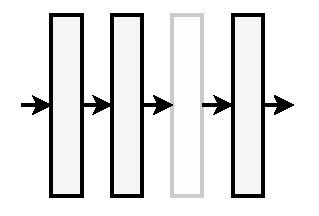
\includegraphics[width=1.0\textwidth]{images/gradient_checkpointing-Pagina-1}
    \caption{}
    \end{subfigure}
    \hfill
    \begin{subfigure}[b]{0.23\textwidth}
    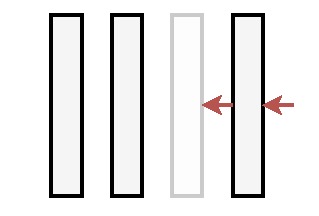
\includegraphics[width=1.0\textwidth]{images/gradient_checkpointing-Pagina-2}
    \caption{}
    \end{subfigure}
    \hfill
    \begin{subfigure}[b]{0.23\textwidth}
    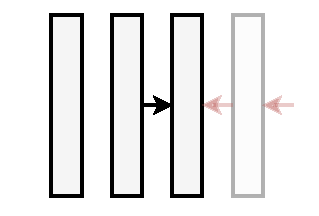
\includegraphics[width=1.0\textwidth]{images/gradient_checkpointing-Pagina-3}
    \caption{}
    \end{subfigure}
    \hfill
    \begin{subfigure}[b]{0.23\textwidth}
    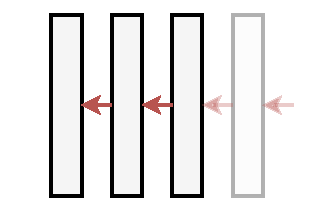
\includegraphics[width=1.0\textwidth]{images/gradient_checkpointing-Pagina-4}
    \caption{}
    \end{subfigure}
    \hfill
    \caption{Пример \textbf{чекпоинтинга градиентов}. (a) Мы выполняем прямой проход, но сохраняем только выходы первого, второго и четвертого блоков (\textbf{чекпоинты}). (b) Обратный проход (красные стрелки) останавливается на третьем блоке, активации которого недоступны. (c) Мы запускаем второй прямой проход, начиная с ближайшего чекпоинта, чтобы снова материализовать активации. (d) Мы завершаем прямой проход. По сравнению со стандартным обратным проходом, это требует в 1.25 раза больше вычислений. В общем, чем меньше сохраняется чекпоинтов, тем выше вычислительная стоимость обратного прохода.}
    \label{fig:gradient_checkpointing}
\end{figure}

\section{Практические соображения}

\subsection{Векторно-якобианские произведения}

Глядя на шаг (3) в алгоритме R-AD, мы можем сделать интересное наблюдение: единственная операция, которая нам нужна, — это произведение вектора-строки $\mathbf{v}$ на Якобиан $f$ (либо входной, либо весовой Якобиан). Мы называем эти две операции \textbf{векторно-якобианскими произведениями} (VJP) $f$.\footnote{В отличие от этого, F-AD можно сформулировать полностью в терминах транспонированного VJP, называемого \textbf{якобиан-векторным произведением} (JVP). Для одномерного выхода JVP — это производная по направлению \eqref{eq:directional_derivative} из Раздела \ref{sec:gradients_and_jacobians}. Всегда по аналогии, VJP представляет собой применение линейного отображения, связанного с бесконечно малыми вариациями \textit{выхода} функции, см. \cite{blondel2024elements}.} В следующем определении мы восстанавливаем размерную согласованность, добавляя транспонирование к вектору.

\begin{definition}[Векторно-якобианское произведение (VJP)] \addbottle
    Для функции $\mathbf{y}=f(\mathbf{x})$, где $\mathbf{x} \sim (c)$ и $\mathbf{y} \sim (c^\prime)$, ее VJP — это другая функция, определяемая как:
    %
    \begin{equation}
    \textnormal{vjp}_f(\mathbf{v})=\mathbf{v}^\top \partial f(\mathbf{x})
    \end{equation}
    %
    где $\mathbf{v}\sim (c^\prime)$. Если $f$ имеет несколько параметров $f(\mathbf{x}_1, \ldots, \mathbf{x}_n)$, мы можем определить $n$ отдельных VJP, обозначаемых как $\textnormal{vjp}_{f,\mathbf{x}_1}(\mathbf{v})$, ..., $\textnormal{vjp}_{f, \mathbf{x}_n}(\mathbf{v})$.
\end{definition}

В частности, в нашем случае мы можем определить два типа VJP, соответствующие входному и весовому аргументам соответственно:
%
\begin{gather}
\text{vjp}_{f,\mathbf{x}}(\mathbf{v})=\mathbf{v}^\top\partial_\mathbf{x}f(\mathbf{x},\mathbf{w}) \label{eq:input_jacobian}\\
\text{vjp}_{f, \mathbf{w}}(\mathbf{v})=\mathbf{v}^\top\partial_\mathbf{w}f(\mathbf{x},\mathbf{w})\label{eq:weight_jacobian}
\end{gather}
%
Теперь мы можем переписать две операции на шаге (3) алгоритма R-AD как два вызова VJP примитивной функции с сопряженными значениями (игнорируя индексы $i$ для удобочитаемости), соответствующие сопряженному, умноженному на весовой VJP, и сопряженному, умноженному на входной VJP:
%
\begin{gather}
\partial_{\mathbf{w}} \, y = \text{vjp}_{f,\mathbf{w}}\left(\widetilde{\mathbf{h}}\right) \label{eq:r_ad_1}\\
\widetilde{\mathbf{h}}  \gets \text{vjp}_{f, \mathbf{h}}\left(\widetilde{\mathbf{h}}\right) \label{eq:r_ad_2}
\end{gather}
%
Следовательно, мы можем реализовать целую систему автоматического дифференцирования, сначала выбрав набор примитивных операций, а затем дополнив их соответствующими VJP, без необходимости материализовать Якобианы в памяти в какой-либо момент. Это схематически показано на Рисунке \ref{fig:backward_pass}. 

\begin{SCfigure}
    \centering
    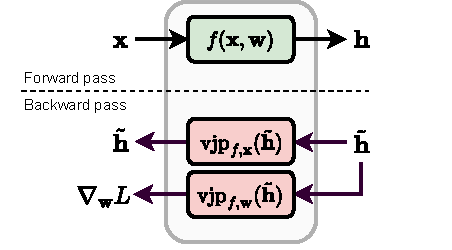
\includegraphics[width=0.55\textwidth]{images/backward_pass-Pagina-2.pdf}
    \caption{Для выполнения R-AD примитивы должны быть дополнены двумя операциями VJP, чтобы можно было выполнить обратный проход, соответствующий входному VJP \eqref{eq:input_jacobian} и весовому VJP \eqref{eq:weight_jacobian}. Одного вызова для каждой достаточно для выполнения обратного прохода через примитив, что соответствует \eqref{eq:r_ad_1}-\eqref{eq:r_ad_2}.}
    \label{fig:backward_pass}
\end{SCfigure}

Фактически, мы можем восстановить вычисление Якобианов, многократно вызывая VJP с базисными векторами $\mathbf{e}_1, \ldots, \mathbf{e}_n$, чтобы генерировать их по одной строке за раз, например, для входного Якобиана мы имеем:
%
$$\partial_{\mathbf{x}}f(\mathbf{x},\mathbf{w})=\begin{bmatrix} \text{vjp}_{f,\mathbf{x}}(\mathbf{e}_1) \\ \text{vjp}_{f,\mathbf{x}}(\mathbf{e}_2) \\ \vdots\\ \text{vjp}_{f,\mathbf{x}}(
\mathbf{e}_n) \end{bmatrix}$$
%
Чтобы понять, почему эта переформулировка может быть удобной, давайте посмотрим на VJP полносвязного слоя, который состоит из линейных проекций и (поэлементных) нелинейностей. Во-первых, рассмотрим простую линейную проекцию без смещения:
%
$$
f(\mathbf{x}, \mathbf{W})=\mathbf{W}\mathbf{x}
$$
%
Входной Якобиан здесь — это просто $\mathbf{W}$, но весовой Якобиан — это тензор 3-го ранга (Раздел \ref{sec:gradients_and_jacobians}). Для сравнения, входной VJP не имеет особой структуры:
%
\begin{equation}
\text{vjp}_{f, \mathbf{x}}(\mathbf{v})=\mathbf{v}^\top\mathbf{W}^\top = \left[\mathbf{W}\mathbf{v}\right]^\top
\label{eq:vjp_x_matrix_multiplication}
\end{equation}
%
Весовой VJP, напротив, оказывается простым внешним произведением, что полностью избегает тензоров 3-го ранга:
%
\begin{equation}
\text{vjp}_{f,\mathbf{w}}(\mathbf{v}) = \mathbf{v}\mathbf{x}^\top
\label{eq:vjp_w_matrix_multiplication}
\end{equation}
%
\begin{supportbox}{Вычисление VJP}
Чтобы вычислить \eqref{eq:vjp_w_matrix_multiplication}, мы можем записать $y=\mathbf{v}^\top \mathbf{W}\mathbf{x} =\sum_i\sum_j W_{ij}v_ix_j$, откуда мы немедленно получаем $\frac{\partial y}{\partial W_{ij}} = v_ix_j$, что является поэлементным определением внешнего произведения.
\end{supportbox}
%
Следовательно, каждый раз, когда мы применяем линейную проекцию в прямом проходе, мы изменяем обратно распространенные градиенты на транспонированную матрицу ее весов и выполняем внешнее произведение для вычисления градиента $\mathbf{W}$. 

Рассмотрим теперь поэлементную функцию активации без обучаемых параметров, например, ReLU:
%
$$
f(\mathbf{x},\left\{\right\})=\phi(\mathbf{x})
$$
%
Поскольку у нас нет обучаемых параметров, нам нужно рассматривать только входной VJP. Градиент — это диагональная матрица, элементами которой являются производные $\phi$:
%
$$\idx{\partial_{\mathbf{x}} \phi(\mathbf{x})}{ii}=\phi^\prime(x_i)$$
%
Входной VJP — это умножение диагональной матрицы на вектор, что эквивалентно произведению Адамара (т.е. операции масштабирования):
%
\begin{equation}
\text{vjp}_{\mathbf{x}}(f,\mathbf{v})=\mathbf{v}\odot \phi^\prime(\mathbf{x})
\label{eq:backward_pass_activation_function}
\end{equation}
%
Интересно, что и в этом случае мы можем вычислить VJP, не материализуя полную диагональную матрицу.

\subsection{Реализация системы R-AD}
\label{subsec:implementing_rad}
%
Существует много способов реализации системы R-AD, от списков Венгерта (как это сделано в TensorFlow) до преобразований исходного кода в исходный код \cite{griewank2008evaluating}. Здесь мы кратко обсудим некоторые распространенные реализации в существующих фреймворках. 

Во-первых, описание примитивов как функций с двумя аргументами $f(\mathbf{x}, \mathbf{w})$ согласуется с функциональными фреймворками, такими как JAX, где все является функцией. Рассмотрим функцию $f(\mathbf{x})$ с $c$-мерным входом и $c^\prime$-мерным выходом. С этой точки зрения VJP можно реализовать как функцию высшего порядка с сигнатурой:

\begin{mypy}{Вычисление градиента как функция высшего порядка. Интерфейс {\footnotesize\mintinline{python}{torch.func}} воспроизводит API JAX. На практике функцию можно \textit{трассировать} (например, с помощью {\footnotesize\mintinline{python}{torch.compile}}), чтобы сгенерировать оптимизированный вычислительный граф.}{code:functional_grad}
# Исходная функция (сумма квадратов)
def f(x: Float[Array, "c"]):
  return (x**2).sum()

grad_f = func.grad(f)
print(grad_f(torch.randn(10)).shape) 
# [Out]: torch.Size([10])
\end{mypy}

\begin{equation}
(\mathbb{R}^c \rightarrow \mathbb{R}^{c^\prime}) \rightarrow \mathbb{R}^c \rightarrow (\mathbb{R}^{c^\prime} \rightarrow \mathbb{R}^c)
\end{equation}
%
т.е. для функции $f$ и входа $\mathbf{x}^\prime$ VJP возвращает другую функцию, которую можно применить к $c^\prime$-мерному вектору $\mathbf{v}$, чтобы вернуть $\mathbf{v}^\top \partial f(\mathbf{x}^\prime)$. Аналогично, градиент для одномерной функции можно реализовать как другую функцию высшего порядка с сигнатурой:
%
\begin{equation}
(\mathbb{R}^c \rightarrow \mathbb{R}) \rightarrow (\mathbb{R}^c \rightarrow \mathbb{R}^c)
\end{equation}
%
принимая на вход функцию $f(\mathbf{x})$ и возвращая другую функцию, которая вычисляет $\nabla f(\mathbf{x})$. В JAX эти идеи реализованы в функциях {\footnotesize\mintinline{python}{jax.grad}} и {\footnotesize\mintinline{python}{jax.jvp}} соответственно, что также воспроизведено в PyTorch в модуле {\footnotesize\mintinline{python}{torch.func}} - см. Листинг \ref{code:functional_grad} для примера.\footnote{Многие операции, такие как вычисление Гессиана, могут быть достигнуты путем умной композиции JVP и VJP на основе их сигнатур: \url{https://jax.readthedocs.io/en/latest/notebooks/autodiff_cookbook.html}.}

Как мы уже упоминали, на практике наши модели реализованы как композиции объектов, параметры которых инкапсулированы как свойства (Листинг \ref{code:fully_connected_layer}). Одна из возможностей — «очистить» объект, чтобы превратить его в чистую функцию, например:\footnote{\url{https://sjmielke.com/jax-purify.htm}}

{\footnotesize
\begin{minted}{python}
# Извлечение параметров
params = dict(model.named_parameters())
# Функциональный вызов прямой функции модели
y = torch.func.functional_call(model, params, x)
\end{minted}
}

\begin{figure}
    \centering
    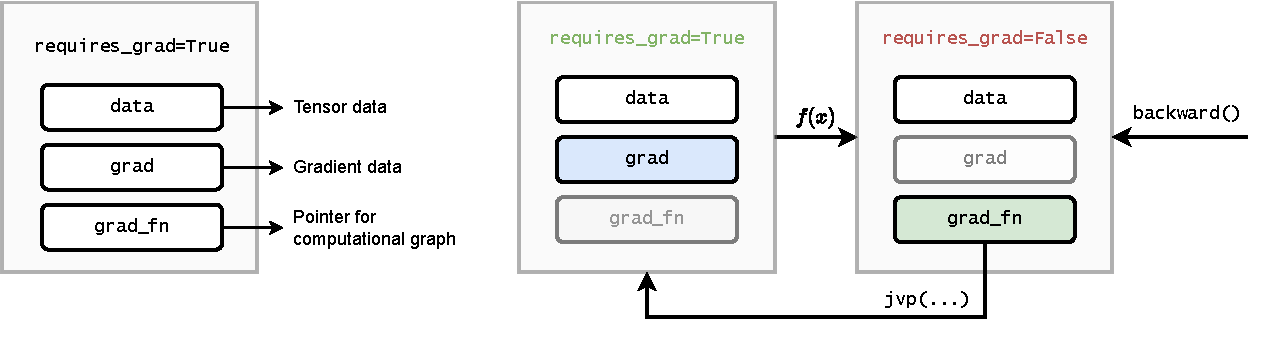
\includegraphics[width=\textwidth]{images/pytorch_wrapper-Pagina-2}
    \caption{Слева: в PyTorch тензор дополняется информацией о его градиенте (пустом при инициализации) и об операции, которая его создала. Справа: во время обратного прохода свойство {\footnotesize\mintinline{python}{grad_fn}} используется для обхода вычислительного графа в обратном порядке, и градиенты сохраняются \textit{внутри} свойства {\footnotesize\mintinline{python}{grad}} тензора, когда {\footnotesize\mintinline{python}{requires_grad}} явно установлено в {\footnotesize\mintinline{python}{True}} (чтобы избежать потребления ненужной памяти).}
    \label{fig:pytorch_wrapper}
\end{figure}

В более общем смысле, фреймворки, такие как PyTorch, дополнены техниками для прямой обработки этого сценария, без введения промежуточных операций. В PyTorch, например, объекты тензоров дополняются информацией об операции, которая их сгенерировала (Рисунок \ref{fig:pytorch_wrapper}, слева). Всякий раз, когда запрашивается вызов {\footnotesize\mintinline{python}{backward()}} для скалярного значения, эти свойства используются для обхода вычислительного графа в обратном порядке, сохраняя соответствующие градиенты \textit{внутри} тензоров, которые их требуют (Рисунок \ref{fig:pytorch_wrapper}, справа). 

Это лишь общий обзор того, как эти системы реализованы на практике, и мы оставляем за скобками многие детали, за которыми мы отсылаем к официальной документации.\footnote{Я определенно рекомендую попробовать реализовать систему R-AD с нуля: в Интернете можно найти много дидактических реализаций, например, \url{https://github.com/karpathy/micrograd}.}

\subsection{Выбор функции активации}

По совпадению, теперь мы можем обосновать, почему ReLU является хорошим выбором в качестве функции активации. Внимательный взгляд на \eqref{eq:backward_pass_activation_function} говорит нам, что каждый раз, когда мы добавляем функцию активации в нашу модель, сопряженные значения в обратном проходе масштабируются на коэффициент $\phi^\prime(\mathbf{x})$. Для моделей с большим количеством слоев это может привести к двум патологическим поведениям:

\begin{enumerate}
\item Если $\phi^\prime(\cdot) < 1$ везде, существует риск того, что градиент будет экспоненциально быстро уменьшаться до 0 с увеличением числа слоев. Это называется проблемой \textbf{исчезающего градиента}.
\item И наоборот, если $\phi^\prime(\cdot) > 1$ везде, возникает противоположная проблема, когда градиенты экспоненциально сходятся к бесконечности с увеличением числа слоев. Это называется проблемой \textbf{взрывающегося градиента}.
\end{enumerate}

На практике это серьезные проблемы, поскольку библиотеки представляют числа с плавающей запятой с ограниченной точностью (обычно 32 бита или меньше), что означает, что при увеличении числа слоев быстро могут возникать потери точности или переполнения.

\begin{supportbox}{Линейные нелинейные модели}
Удивительно, но стек линейных слоев, реализованный с точностью с плавающей запятой, не является полностью линейным из-за небольших разрывов на машинной точности! Обычно это не проблема, но это можно использовать для обучения полностью линейных глубоких нейронных сетей.\footnote{\url{https://openai.com/research/nonlinear-computation-in-deep-linear-networks}.}
\end{supportbox}

В качестве примера того, как могут возникать исчезающие градиенты, рассмотрим функцию сигмоида $\sigma(s)$. Мы уже упоминали, что в прошлом это была распространенная ФА, поскольку она является мягкой аппроксимацией ступенчатой функции. Мы также знаем, что $\sigma^\prime(s)=\sigma(s)(1-\sigma(s))$. В сочетании с тем фактом, что $\sigma(s) \in \left[0,1\right]$, мы получаем, что:
%
$$\sigma^\prime(s)\in\left[0,0.25\right]$$
%
Следовательно, сигмоида является главным кандидатом на проблемы с исчезающим градиентом: см. Рисунок \ref{fig:sigmoid_and_derivative}.

\begin{figure}
    \centering
    \begin{subfigure}[b]{0.48\textwidth}
    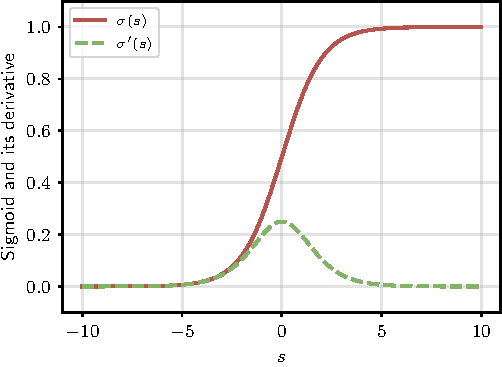
\includegraphics[width=1.0\textwidth]{images/sigmoid_and_derivative}
    \caption{Сигмоида}
    \label{fig:sigmoid_and_derivative}
    \end{subfigure}
    \hfill
    \begin{subfigure}[b]{0.48\textwidth}
    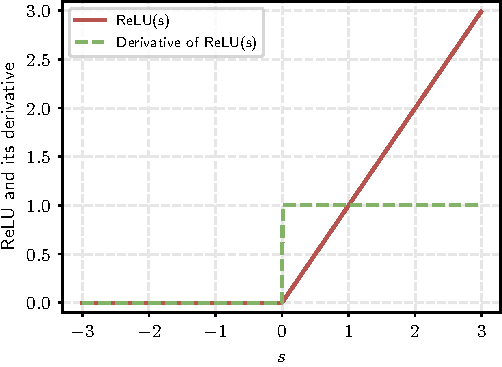
\includegraphics[width=1.0\textwidth]{images/relu_and_derivative}
    \caption{ReLU}
    \label{fig:relu_and_derivative}
    \end{subfigure}
    \caption{(a) График функции сигмоида ({\color{drawred}красный}) и ее производной ({\color{drawgreen}зеленый}). (b) График ReLU ({\color{drawred}красный}) и ее производной ({\color{drawgreen}зеленый}).}
\end{figure}

Разработка ФА, которая никогда не демонстрирует исчезающих или взрывающихся градиентов, нетривиальна, поскольку единственная функция, имеющая $\phi^\prime(s)=1$ везде, — это постоянная функция. Тогда нам нужна функция, которая является «достаточно линейной», чтобы избежать проблем с градиентом, но «достаточно нелинейной», чтобы разделять линейные слои. ReLU оказывается хорошим кандидатом, поскольку:
%
$$\partial_s \text{ReLU}(s)=\begin{cases} 0 & s < 0 \\ 1 & s >0 \end{cases}$$
%
Градиент либо обнуляется, вызывая разреженность в вычислениях, либо умножается на $1$, избегая проблем с масштабированием - это показано на Рисунке \ref{fig:relu_and_derivative}.

В качестве примечания, градиент ReLU идентичен независимо от того, заменяем ли мы вход в слой ReLU его выходом (поскольку мы только маскируем отрицательные значения, сохраняя положительные значения без изменений). Следовательно, еще одним преимуществом использования ReLU в качестве функции активации является то, что мы можем сэкономить немного памяти при выполнении R-AD, перезаписывая вход слоя в прямом проходе, не влияя на правильность процедуры AD: это делается в PyTorch, например, путем установки параметра {\footnotesize\verb+in_place+}.\footnote{\url{https://pytorch.org/docs/stable/generated/torch.nn.ReLU.html}.}

\subsection{Субдифференцируемость и корректность АД}
\label{subsec:subdifferentiability}

\addteacup Есть небольшая деталь, которую мы до сих пор избегали обсуждать: ReLU недифференцируема в $0$, что делает общую сеть негладкой. Что происходит в этом случае? «Прагматичный» ответ заключается в том, что при минимизации с помощью стохастического градиентного спуска из случайной (ненулевой) инициализации вероятность оказаться точно в $s=0$ практически равна нулю, в то время как градиент определен в $\text{ReLU}(\varepsilon)$ для любого $\lvert\varepsilon\rvert>0$.

Для более технического ответа мы можем ввести понятие \textbf{субградиента} функции.

\begin{definition}[Субградиент]
%
Для выпуклой функции $f(x)$ субградиент в $x$ — это точка $z$, такая, что для всех $y$:
%
$$
f(y) \ge f(x)+z(y-x)
$$
%
\end{definition}

Обратите внимание на сходство с определением выпуклости: субградиент — это наклон прямой, «касательной» к $f(x)$, такой, что вся $f$ ограничена ею снизу. Если $f$ дифференцируема в $x$, то существует только одна такая прямая, которая является производной $f$ в $x$. В негладкой точке существует несколько субградиентов, и они образуют множество, называемое \textbf{субдифференциалом} $f$ в $x$:
%
$$\partial_x f(x)=\left\{z \,\vert\, z \text{ является субградиентом } f(x)\right\}$$

С этим определением в руках мы можем завершить наш анализ градиента ReLU, заменив градиент его субдифференциалом в $0$:
%
$$\partial_s \text{ReLU}(s)=\begin{cases} \left\{0\right\} & s < 0 \\ \left\{1\right\} & s >0 \\ \left[0,1\right] & s=0 \end{cases}$$
%
Следовательно, любое значение в $[0,1]$ является допустимым субградиентом в $0$, причем большинство реализаций на практике предпочитают $\text{ReLU}^\prime(0)=0$. Выбор субградиентов на каждом шаге итерационной процедуры спуска называется \textbf{субградиентным спуском}. 

На самом деле, ситуация еще сложнее, потому что субградиент не обязательно определен для невыпуклых функций. В этом случае можно прибегнуть к обобщениям, которые ослабляют предыдущее определение до локальной окрестности $x$, таким как субдифференциал Кларка.\footnote{\url{https://en.wikipedia.org/wiki/Clarke_generalized_derivative}} Субдифференцируемость также может создавать проблемы в АД, где разные реализации одних и тех же функций могут давать разные (возможно, неверные) субградиенты, и для формального доказательства необходимо рассматривать более уточненные концепции цепных правил \cite{kakade2018provably,bolte2020mathematical}.\footnote{Рассмотрим этот пример, воспроизведенный из \cite{bolte2020mathematical}: определим две функции, $\text{ReLU}_2(s) = \text{ReLU}(-s)+s$ и $\text{ReLU}_3(s) = 0.5(\text{ReLU}(s)+\text{ReLU}_2(s))$. Они обе эквивалентны ReLU, но в PyTorch обратный проход в $0$ возвращает $0.0$ для ReLU, $1.0$ для ReLU$_2$ и $0.5$ для ReLU$_3$.}

\section*{От теории к практике}

\begin{wrapfigure}{r}{3.0cm}
\vspace{-3em}
\includegraphics[width=3.0cm]{images/shutterstock_2075221579.jpg}
\vspace{-3em}
\end{wrapfigure}

Если вы следовали упражнениям в Главе \ref{chap:fully_connected_models}, вы уже видели применение R-AD как в PyTorch, так и в JAX, и эта глава (особенно Раздел \ref{subsec:implementing_rad}) должна была прояснить их реализацию.

Хорошая идея — попробовать перереализовать простую систему R-AD, похожую на ту, что в PyTorch. Например, сосредоточившись на скалярных величинах, репозиторий \texttt{micrograd}\footnote{\url{https://github.com/karpathy/micrograd}} является очень хорошей дидактической реализацией. Единственная деталь, которую мы не рассматриваем, заключается в том, что, как только вы переходите к общему ациклическому графу, упорядочение переменных в вычислительном графе перед обратным проходом необходимо, чтобы избежать создания неверных путей обратного распространения. В micrograd это достигается с помощью недорогой топологической сортировки переменных.

Также интересно попробовать реализовать новый примитив (в смысле, используемом в этой главе) в PyTorch, что требует указания его прямого прохода вместе с его JVP.\footnote{\url{https://pytorch.org/docs/master/notes/extending.html}}
Одним из примеров может быть одна из обучаемых функций активации из Раздела \ref{sec:activation_functions}. Это дидактическое упражнение, в том смысле, что это можно реализовать эквивалентно, подклассифицируя \mintinline{python}{nn.Module} и позволяя движку AD PyTorch вычислить обратный проход.

Все эти шаги также можно воспроизвести в JAX:
\begin{itemize}
\item Реализуйте дидактическую версию JAX с помощью \texttt{autodidax}: \url{https://jax.readthedocs.io/en/latest/autodidax.html}
\item Напишите новый примитив, реализовав соответствующий VJP: \url{https://jax.readthedocs.io/en/latest/notebooks/Custom_derivative_rules_for_Python_code.html}
\item Прочтите \textbf{JAX Autodiff} Cookbook\footnote{\url{https://jax.readthedocs.io/en/latest/notebooks/autodiff_cookbook.html}}, чтобы узнать о расширенных вариантах использования движка автоматического дифференцирования, таких как производные высшего порядка, Гессианы и многое другое. 
\end{itemize}